%---------------------------------------------------------------------------------------------------
% Introduction
%---------------------------------------------------------------------------------------------------
\newpage
%\part{start}
\chapter{Introduction}
    \section{Multi Agent Resource And Simulation}
        \label{section:MARS}
        The MARS\footnote{MARS: Multi Agent Research and Simulation} Group is a simulation framework developed 
        in HAW Hamburg as a  part of the student research project. The project can be classified as a
        Distributed System \cite{DistributedSystems} designed to carry out simulations of a given model 
        \cite{HAWHamburgMARS}. 
        A model describes a digital prototype of a physical agents i.e wolves, sheep, grass etc 
        which can be simulated to predict a real world scenario. A simple model would
        be the wolves and sheep, using this prototype one can simulate the interaction between the agents. 
        As a result one can analyze the population change between them for this model. 

        \par
        To leverage the MARS framework in executing a simulation, specific steps have to be 
        carried out in a chronological manner which are as follows. 
        \begin{enumerate}
            \item 
                \textbf{Create a project}: A project can be defined as a collection of all the resources
                and the simulation results. The resources include models,  scenario description, result configurations, simulation plans,
                simulation runs, simulation results and different files required by the model
                like GIS\footnote{\label{footnote:GIS}GIS: Geographic Information System} Layers \cite[p.~1]{{GIS}}
                Time series \cite{Timeseries} layer etc.
            \item
                \textbf{Upload models and corresponding files}:  The model upload is the first step required
                for a simulation to take place. The model contains information about how the agents behave
                during a simulation run. A model can also be dependent upon other files such as 
                GIS Layers \cite[p.~1]{{GIS}} , Time series \cite{Timeseries} Layer etc, where they are 
                uploaded separately. 

            \item 
                \textbf{Create a scenario}: A scenario of a project can be described as the initialization of the model.
                In process of creating a scenario, attributes like number of agents i.e. wolves, sheep are specified, 
                the uploaded layers like the GIS, Time series etc, if required, are assigned to the model. Also,
                the execution duration parameters of the simulation run are configured.

            \item 
                \textbf{Configure result configuration}: The result configuration enables the user to choose
                the agents desired to be executed in the simulation. This means in the result 
                configuration, one can turn off the 'wolves' output in the Wolves and Sheep models.
            \item  
                \textbf{Create simulation plan and run}: A simulation plan is a complete description of the
                 simulation which includes, scenario and result configuration. For the execution of a simulation
                 one must run the simulation plan, which creates
                 a simulation run. A simulation run contains all the metadata i.e. simulation id, simulation 
                 job status i.e. running, failed, creating etc. Using the simulation run one can analyze the 
                 simulation results.
        \end{enumerate} 
        
        \begin{figure}[H]
            \centering 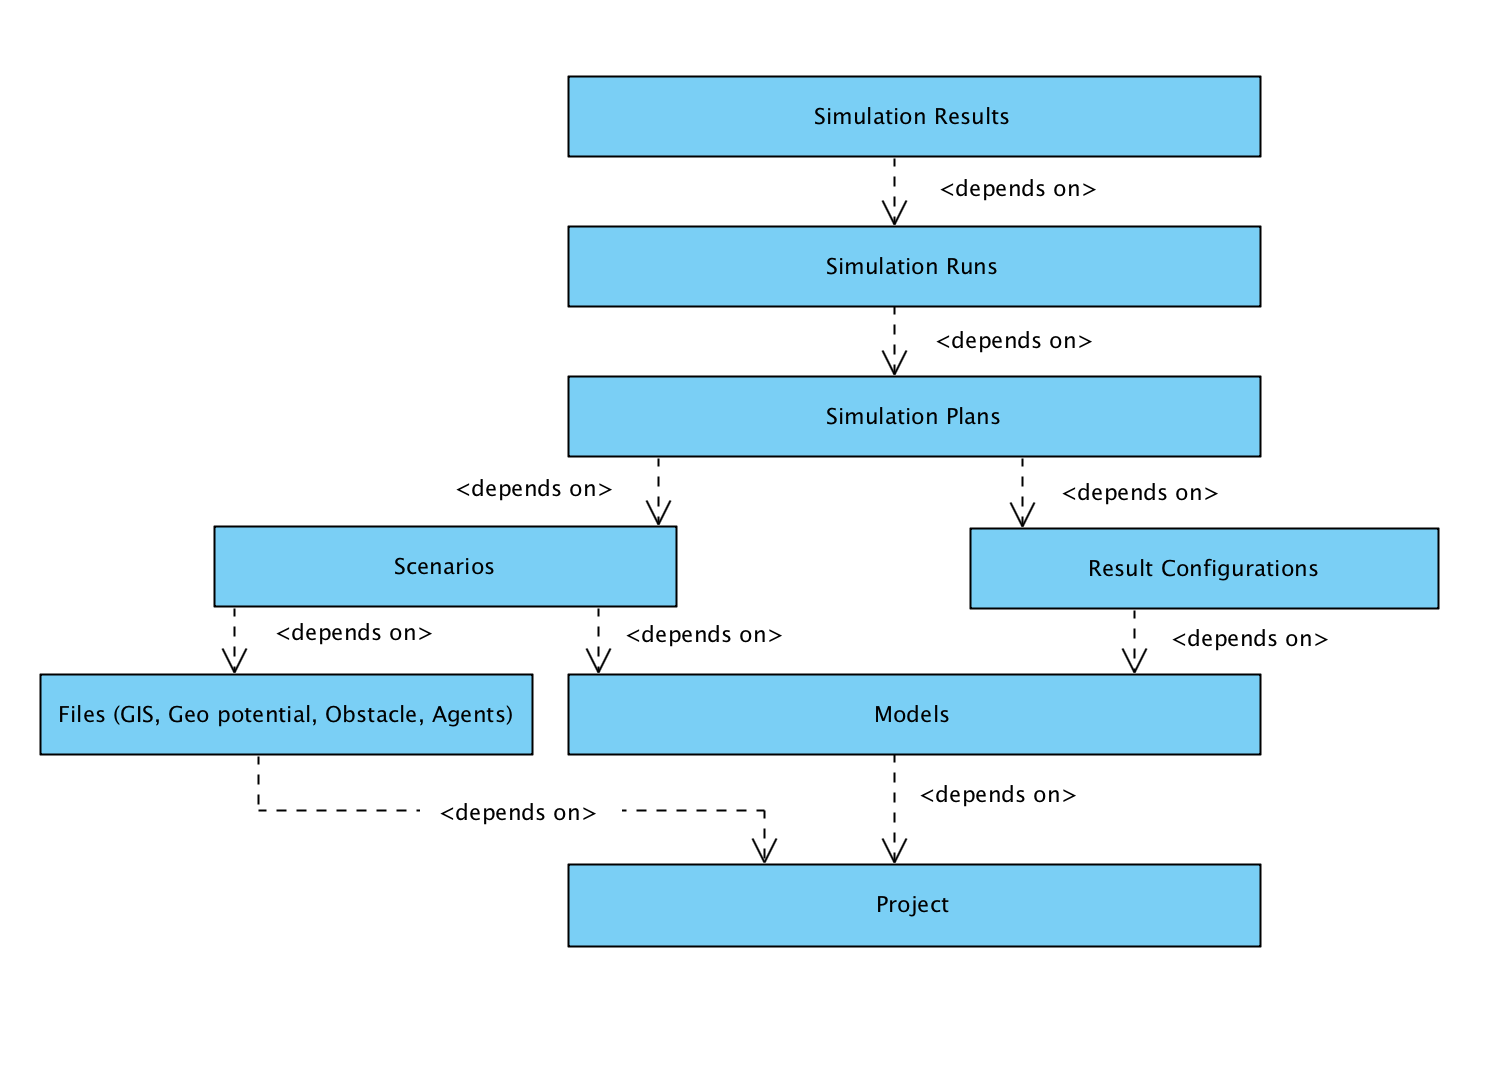
\includegraphics[scale=0.6]{grafiken/marsDependency.png}
            \caption{MARS Resource UML dependency graph}
            \label{fig:marsDependency}
        \end{figure}
        
        Figure \ref{fig:marsDependency} shows how the MARS\footnote{MARS: Multi Agent Research and Simulation} 
        resources are dependent. It can be observed
        that the order of existence of the resources have to be from the project to the simulation results 
        (bottom to top) when adding a new simulation. Failure to follow this graph will result in failure to
        successfully run a simulation.

        \begin{figure}[H]
            \centering 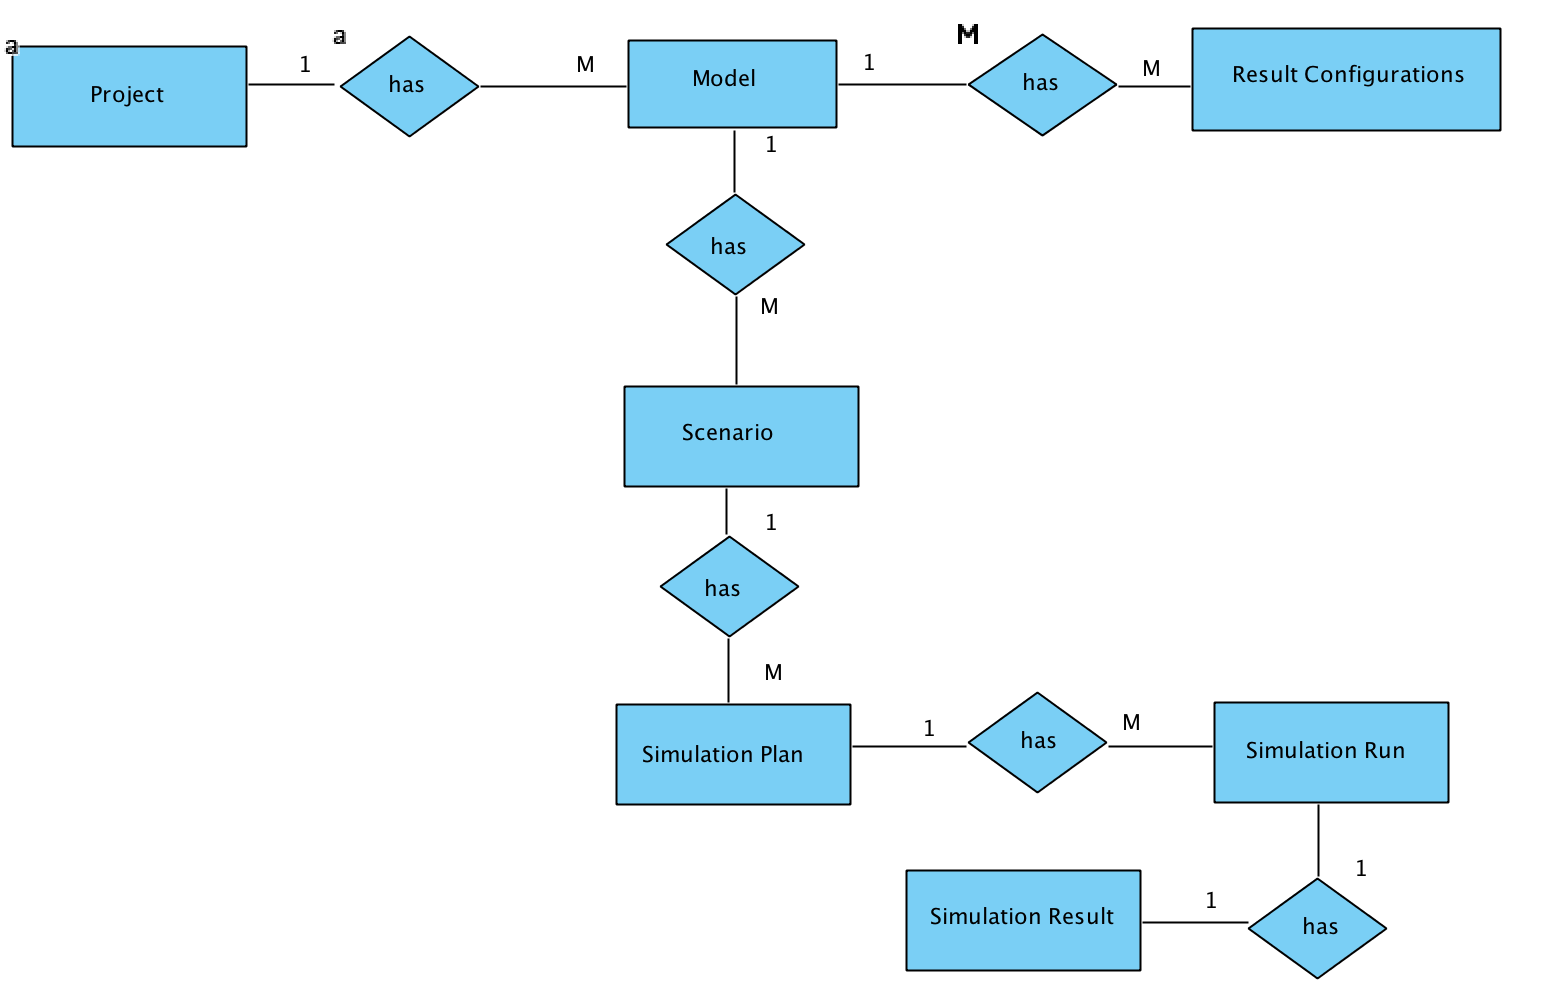
\includegraphics[scale=0.6]{grafiken/ERMars.png}
            \caption{Chen notation Entity Relation Diagram for MARS resources}
            \label{fig:ERMars}
        \end{figure}
        
        From Figure \ref{fig:marsDependency} a tight dependency between the resources can be witnessed,  
        as one resource does not make sense to exist without the dependent resource. 
        Hence, it can be argued that the entities, Model, result configurations, scenario, simulation plans, 
        simulation runs and simulation results should be a weak entity in the Entity-Relation Diagram. This is not
        the case here because except for the project all the other resources are stored in a NoSql database
        called "Mongo DB" \cite{MongoDB}. Since NoSql technology has no tables and does not need to make joins,
        the resources can exist independently. This is the reason why the coupled entities are not chosen to 
        be a weak entity.

        \newpage
         

        \begin{table}[h!]
            \centering
            \begin{tabular}{|p{3cm}|p{11cm}|}
                \hline
                    \textbf{Service Name}  & \textbf{Description}\\
                \hline
                    Project Service & 
                    A mature team must be present to maintain large number of services \\
                \hline
                    File Service
                    & All the services must manage eventual consistency which is
                    harder to manage in a large distributed system.\\
                \hline
                    Scenario Service  & Harder to program since remote calls must be made.\\
                \hline
            \end{tabular}
            \caption{Advantages and disadvantages of microservices \cite{FowlerMartin}}
            \label{table:Advantages and disadvantages of microservices}     
        \end{table}    

    \section{Problem Statement}

        The main aim of this thesis is to design and test an archive service
        to the existing MARS system. This service's responsibility is to move the related resources.The archived data is intended 
        to be used for future research purposes.
        The MARS is a complex distributed network having an
        hierarchal dependency with the co-existing microservices. The system being designed
        in such an architecture entails one service to be tightly coupled with one other. It is 
        a big challenge, since great amount of care should be taken into consideration of how the 
        data are being stored and the order for retrieval of the data back into the active system.
        This service will be a supporting tool for further development of the system to become more 
        efficient and compliant. 
         
    
    \section{Motivation}
    
        The MARS\footnotemark system produces simulation results of 
        different models i.e. simulation of wolves eating sheep. Depending upon the 
        configuration and the model a random output is generated. The size of the produced
        output can vary from kilobytes to terabytes of data. As the system grows older the 
        number of simulation runs and the output produced are going to increase. The increase
        of the number of resources in the active entity causes performance to hinder. 
        A very high level of correlation has been observed between the operating cost of a software 
        system and its data volume. 
        
   
        \par

        At the time of writing this thesis, the output data and the project data are stored in a
        SEV file system \cite{SEV}. This provides a faster and efficient method for data
        access but this storage is rather expensive to get more volume. Due to the financial cost 
        factor the primary storage volume available is very limited. Since the simulation 
        results are random in nature, it is a point of interest to keep the data for future
        research purposes with its configurations. With archiving service in hand to the system, 
        it would be possible to move the inactive or selected projects to the secondary storage. 
        The secondary storage is larger in volume and cheaper. 
        
        \par

        For the MARS\footnotemark[\value{footnote}] project, this serves as enormous
        motivation to introduce a service which would archive the chosen project
        into another cheaper storage component available, in this case NAS synology 
        \cite{Synology}. Having such a service included would maintain a positive impact 
        towards the reliability and robustness of the system by having less data in the 
        active system and thus have fewer operations to be executed.
        
        \footnotetext{Multi Agent Research and Simulation}    


    

    \section{Thesis Overview}
        Here is a brief description of the thesis, providing a short overview on what each
        chapter contains.
        
        \par
        \textbf{Chapter 2: "Theory"}, this chapter describes about the design
        of the MARS system, the hierarchal structure of the services and the technologies used to
        deploy it.

        \par
        \textbf{Chapter 3: "Requirement Analysis"}, this chapter describes the functional and
        non-functional objectives of the archive service.

        \par
        \textbf{Chapter 4: "Design Of The Solution"}, this chapter explains in detail, the 
        methodologies for data storage, archive process and the software design.

        \par
        \textbf{Chapter 5: "Implementation"}, this chapter is where the details of the 
        implementation decision are explained.

        \par
        \textbf{Chapter 6: "Result And Validation"}, this chapter explains in details about 
        some test cases and result validation that were carried out.

        \par
        \textbf{Chapter 7: "Conclusion"}, this chapter presents the outcomes and some 
        suggestions for improvements which can be applied.
        
        \par
        \textbf{Appendix}
        MUST BE WRITTEN

